\documentclass[12pt]{article}

\usepackage{url}
\usepackage{geometry}
\geometry{a4paper}
\usepackage{microtype}

\usepackage{graphicx}
\usepackage{amsmath}
\usepackage{algorithm}
\usepackage[noend]{algpseudocode}
\usepackage{float}
\usepackage{wrapfig}
\usepackage{listings}
\usepackage{multirow}
\usepackage{hyperref}

\usepackage{enumitem}

%para escribir en español
\usepackage[utf8x]{inputenc}
\usepackage[spanish]{babel}

\renewcommand{\contentsname}{Índice}
\renewcommand{\refname}{Referencias}
\renewcommand{\figurename}{Figura}

\usepackage[nottoc,numbib]{tocbibind}

\linespread{1.2}

\graphicspath{{./figures/}} % Specifies the directory where pictures are stored

\begin{document}

\begin{titlepage}

    \center

    \textsc{\LARGE Universidad de la República}\\[1.5cm]
    \textsc{\Large Facultad de Ingeniería}\\[1.0cm]
    \textsc{\large Recuperación de Información y Recomendaciones en la Web}\\[0.5cm]

    \rule{\linewidth}{0.5mm} \\[1cm]
    {\huge \bfseries Amazon Copilot}\\[0.5cm]
    \rule{\linewidth}{0.5mm} \\[1.5cm]

    \begin{minipage}{0.4\textwidth}
        \begin{flushleft} \large
            \emph{Autores:}\\
            Juan Pablo Conde\\
            Xavier Iribarnegaray\\
            Juan Pablo Sotelo\\
        \end{flushleft}
    \end{minipage}
    ~
    \begin{minipage}{0.4\textwidth}
        \begin{flushright} \large
            \emph{Profesores:} \\
            Libertad Tansini \\
        \end{flushright}
    \end{minipage}\\[2cm]

    {\large \today}\\[1.5cm]

    
\includegraphics[width=0.4\textwidth]{fing-logo}\\[1cm]

    \vfill

\end{titlepage}

\pagenumbering{arabic}

\tableofcontents

\newpage

\section{Introducción}
Amazon Copilot constituye un sistema diseñado para optimizar la búsqueda y selección de productos en plataformas de comercio electrónico. Basado en un conjunto de datos de productos de Amazon, el sistema implementará técnicas avanzadas de recuperación de información y procesamiento de lenguaje natural para proporcionar una experiencia de compra intuitiva y personalizada.

El proyecto integra tres funcionalidades principales: un sistema de búsqueda híbrido que combina técnicas semánticas y tradicionales para ofrecer resultados más relevantes; un asistente conversacional (Agente de Inteligencia Artificial) que proporciona una interfaz de búsqueda interactiva, refinando requerimientos mediante diálogo natural y utilizando como mecanismo subyacente el sistema de búsqueda híbrido implementado; y un sistema de recomendación que, basándose en los productos seleccionados en el carrito, emplea el mismo agente para identificar artículos similares o complementarios, mejorando así la experiencia de descubrimiento de productos.

\section{Funcionalidades del Sistema}

En esta sección se presentan las tres principales funcionalidades que se implementarán en Amazon Copilot.

\subsection{Búsqueda Híbrida de Productos}

Este componente combina técnicas de búsqueda semántica con métodos tradicionales de correspondencia textual para optimizar resultados. Incorpora representaciones vectoriales semánticas (embeddings) para capturar el significado contextual de las consultas, mantiene búsqueda por términos exactos para consultas específicas e implementa filtrado por categorías. El sistema ordena los resultados mediante un modelo que pondera tanto la relevancia semántica como la coincidencia sintáctica tradicional, logrando un equilibrio óptimo que aprovecha las fortalezas de ambos enfoques para mostrar los productos más pertinentes al usuario.

\subsection{Búsqueda Conversacional con Agente de IA}

El asistente conversacional proporciona una interfaz de búsqueda interactiva en lenguaje natural. Este agente mantiene el contexto durante la conversación, refina progresivamente los requerimientos del usuario mediante preguntas específicas, y utiliza la API de búsqueda híbrida como herramienta subyacente para ofrecer resultados personalizados. Resulta especialmente útil para usuarios sin conocimientos específicos sobre los productos que buscan.

\subsection{Sistema de Recomendación con Agente de IA}

Este sistema analiza los productos seleccionados en el carrito para sugerir artículos complementarios o alternativos. Opera automáticamente al visualizar el carrito, generando recomendaciones basadas en productos frecuentemente adquiridos conjuntamente y alternativas similares. Presenta explicaciones concisas sobre cada recomendación y adapta las sugerencias dinámicamente según el contenido del carrito y el historial de la conversación con el usuario.

\section{Arquitectura del Sistema}

Esta sección describe los componentes principales del sistema, sus responsabilidades e interacciones, así como las tecnologías propuestas para su implementación.

\vspace{1cm}

\begin{figure}[H]
    \centering
    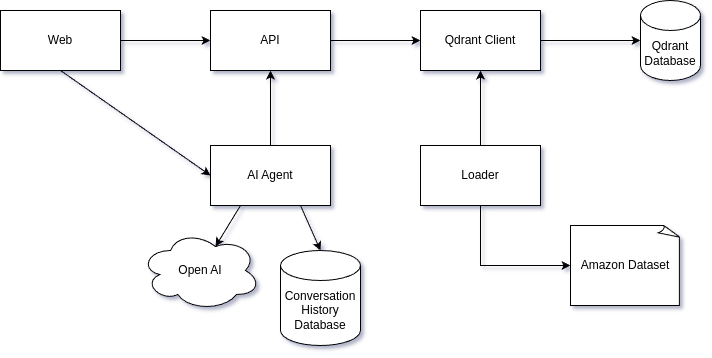
\includegraphics[width=0.8\textwidth]{architecture.png}
    \caption{Diagrama de alto nivel de la arquitectura del sistema.}
    \label{fig:system_architecture}
\end{figure}

\subsection{API}

Este componente constituye la capa de servicios que comunica el frontend con los distintos motores de búsqueda y recomendación. Incluye endpoints para listar productos (recibiendo parámetros de filtros y búsqueda) y para obtener información detallada de productos específicos.

\subsubsection{Implementación}

La API será implementada utilizando \href{https://fastapi.tiangolo.com/}{FastAPI}~\cite{FastAPI}, un framework moderno de Python que permite un desarrollo eficiente y robusto. FastAPI ofrece validación automática de datos mediante \href{https://docs.pydantic.dev/latest/}{Pydantic}~\cite{Pydantic}, tipado estático que reduce errores en tiempo de desarrollo, y generación automática de documentación con OpenAPI y Swagger UI. Esta documentación servirá como recurso valioso para la fase de desarrollo del frontend.

\subsection{Dataset}

Para la información de productos, se utilizará el conjunto de datos de Amazon disponible en \href{https://www.kaggle.com/datasets/lokeshparab/amazon-products-dataset/data?select=Amazon-Products.csv}{Kaggle}~\cite{Amazon}. Este conjunto de datos ofrece una amplia variedad de atributos por producto, incluyendo:

\begin{itemize}
    \item Título y descripción detallada
    \item Categorías y subcategorías
    \item Precio y disponibilidad
    \item Valoraciones y número de reseñas
    \item Imágenes de productos
    \item Especificaciones técnicas
\end{itemize}

La riqueza de estos atributos permitirá implementar las modalidades de búsqueda previamente mencionadas.

\section{Search}

Esta sección describe la implementación técnica del sistema de búsqueda híbrida, desde el procesamiento inicial de datos hasta la ejecución de consultas complejas con filtros y paginación.

\subsection{Procesamiento de Datos Inicial}

El sistema implementa un pipeline robusto de procesamiento de datos que transforma el conjunto de datos original de Amazon en un formato optimizado para búsqueda vectorial. El dataset inicial contiene aproximadamente 550,000 productos, muchos de los cuales presentaban inconsistencias en los datos, imágenes no funcionales o información que requería normalización y limpieza antes de poder ser utilizada efectivamente.

\subsubsection{Limpieza y Normalización}

El proceso de limpieza se ejecuta a través de la función \texttt{clean\_data} en el módulo \texttt{utils.py}, implementando las siguientes transformaciones:

\begin{itemize}
    \item \textbf{Eliminación de valores nulos}: Se descartan productos sin campos esenciales (id, imagen, nombre, categoría, precios)
    \item \textbf{Filtrado de datos inconsistentes}: Se eliminan registros con valoraciones inválidas como \texttt{Get}, \texttt{FREE} o que contengan símbolos no numéricos
    \item \textbf{Normalización de valoraciones}: Conversión de conteos de ratings de formato string con comas a enteros
    \item \textbf{Conversión monetaria}: Transformación automática de precios en rupias indias (INR) a dólares estadounidenses usando tasa de cambio fija
    \item \textbf{Validación de URLs de imágenes}: Verificación concurrente de la accesibilidad de las imágenes de productos
\end{itemize}

\subsection{Base de Datos Vectorial: Qdrant}

La elección de Qdrant como base de datos vectorial se fundamenta en sus capacidades avanzadas para búsqueda híbrida y su arquitectura optimizada para aplicaciones de recuperación de información.

\subsubsection{Justificación Técnica}

Qdrant ofrece ventajas específicas que fueron determinantes para la implementación:

\begin{itemize}
    \item \textbf{Búsqueda híbrida nativa}: Soporte integrado para combinar embeddings densos y esparsos en una sola consulta
    \item \textbf{Modelos de embeddings integrados}: Utilización de FastEmbed para generar representaciones vectoriales sin dependencias externas
    \item \textbf{Filtrado avanzado}: Capacidad de aplicar filtros complejos por categorías, rangos de precios y otros atributos sin impacto significativo en el rendimiento
    \item \textbf{Fácil de usar}: Interfaz intuitiva y documentación clara que facilita la implementación y mantenimiento.
\end{itemize}

\subsubsection{Configuración de la Colección}

La colección se configura con parámetros específicos para optimizar el rendimiento de búsqueda:

\begin{itemize}
    \item \textbf{Vectores densos}: Dimensión 384 con distancia coseno para capturar similitud semántica
    \item \textbf{Vectores esparsos}: Implementación BM25 para coincidencias textuales exactas
    \item \textbf{Índices de payload}: Indexación automática de campos categóricos para filtrado eficiente
\end{itemize}

\subsection{Modelos de Embeddings}

El sistema implementa una arquitectura dual de embeddings que combina representaciones densas y esparsas para maximizar la calidad de los resultados de búsqueda.

\subsubsection{Embeddings Densos: Sentence-Transformers}

Los embeddings densos utilizan el modelo \texttt{sentence-transformers/all-MiniLM-L6-v2}, seleccionado por su balance óptimo entre calidad y eficiencia:

\begin{itemize}
    \item \textbf{Dimensionalidad}: 384 dimensiones que capturan representaciones semánticas ricas con un balance entre precisión, eficiencia y tamaño de los vectores.
    \item \textbf{Entrenamiento}: Pre-entrenado en grandes corpus multilingües.
    \item \textbf{Ventajas}: Excelente para capturar similitudes conceptuales, sinónimos y relaciones semánticas.
\end{itemize}

El proceso de generación de embeddings densos procesa tanto el título como la descripción del producto, creando una representación vectorial que captura el significado semántico completo del artículo.

\subsubsection{Embeddings Esparsos: BM25}

Los embeddings esparsos implementan el algoritmo BM25 a través del modelo \texttt{Qdrant/bm25}, creando representaciones vectoriales donde cada dimensión corresponde a un token específico del diccionario de la colección.

\subsubsection{Estructura del Vector Esparso}

Un embedding esparso se representa como un conjunto de pares (índice, valor) donde:

\begin{itemize}
    \item \textbf{Índice}: Posición del token en el diccionario global de Qdrant para la colección
    \item \textbf{Valor}: Score BM25 que combina la frecuencia del término (TF) con la frecuencia inversa de documento (IDF)
    \item \textbf{Esparsidad}: Solo se almacenan dimensiones con valores no-cero, optimizando el espacio de almacenamiento
\end{itemize}

\subsubsection{Cálculo de Relevancia}

El score BM25 para cada token se calcula mediante la fórmula:

\begin{itemize}
    \item \textbf{Componente TF}: Frecuencia del término normalizada por la longitud del documento usando parámetros k1=1.2 y b=0.75
    \item \textbf{Componente IDF}: Calculado a nivel de colección basado en la frecuencia del término en todos los documentos
    \item \textbf{Actualización dinámica}: Los valores IDF se recalculan automáticamente cuando se añaden nuevos productos a la colección
\end{itemize}

Esta implementación permite:

\begin{itemize}
    \item \textbf{Coincidencias exactas}: Identificación precisa de términos específicos en títulos y descripciones
    \item \textbf{Relevancia estadística}: Ponderación basada en la rareza del término en la colección completa
    \item \textbf{Robustez}: Resistencia a variaciones en la formulación de consultas
    \item \textbf{Eficiencia}: Almacenamiento optimizado que solo mantiene tokens relevantes
\end{itemize}

\subsection{Búsqueda Híbrida}

La implementación de búsqueda híbrida constituye el núcleo del sistema, combinando las fortalezas de ambos tipos de embeddings para proporcionar resultados superiores.

\subsubsection{Principio de Funcionamiento}

La búsqueda híbrida opera ejecutando simultáneamente dos consultas independientes sobre la misma colección de productos:

\begin{itemize}
    \item \textbf{Consulta densa}: Utiliza el embedding denso de la query para encontrar productos semánticamente similares mediante búsqueda por similitud coseno
    \item \textbf{Consulta esparsa}: Aplica el embedding esparso BM25 de la query para identificar productos con coincidencias textuales exactas
    \item \textbf{Ejecución paralela}: Ambas consultas se procesan simultáneamente en Qdrant, optimizando el tiempo de respuesta
    \item \textbf{Aplicación de filtros}: Los filtros de categoría y precio se aplican de manera idéntica a ambas consultas
\end{itemize}

\subsubsection{Ventajas de la Aproximación Dual}

Esta estrategia dual permite capturar diferentes aspectos de la relevancia:

\begin{itemize}
    \item \textbf{Cobertura semántica}: Los embeddings densos identifican productos conceptualmente relacionados aunque no compartan términos exactos
    \item \textbf{Precisión léxica}: Los embeddings esparsos garantizan que productos con términos clave específicos aparezcan en los resultados
    \item \textbf{Compensación mutua}: Cuando una aproximación falla, la otra puede proporcionar resultados relevantes
    \item \textbf{Robustez ante consultas}: El sistema funciona eficazmente tanto para búsquedas conceptuales como específicas
\end{itemize}

\subsubsection{Algoritmo de Fusión}

El sistema implementa una estrategia de fusión que opera en dos niveles:

\begin{itemize}
    \item \textbf{Nivel de puntuación}: Combinación ponderada de scores densos y esparsos usando Reciprocal Rank Fusion (RRF)
    \item \textbf{Normalización}: Ajuste de escalas entre diferentes tipos de scores para comparación equitativa
\end{itemize}

\subsection{Sistema de Filtrado}

El sistema implementa filtros que se aplican tanto a las consultas densas como esparsas durante la búsqueda híbrida.

\subsubsection{Filtros Disponibles}

\begin{itemize}
    \item \textbf{Categoría principal}: Filtrado por categorías como Electronics, Clothing, Home, etc.
    \item \textbf{Subcategoría}: Filtrado de segundo nivel (requiere categoría principal definida)
    \item \textbf{Rango de precios}: Filtros por precio mínimo y/o máximo en dólares
\end{itemize}

\subsubsection{Implementación}

Los filtros utilizan los índices automáticos de Qdrant sobre los campos de payload, aplicándose mediante operadores lógicos AND para combinar múltiples condiciones de filtrado.

\subsection{Paginación}

La implementación de paginación está optimizada para mantener rendimiento consistente independientemente del tamaño del conjunto de resultados.

\subsubsection{Implementación}

El sistema utiliza paginación basada en offset con optimizaciones específicas:

\begin{itemize}
    \item \textbf{Offset y limit}: Parámetros estándar para control granular de resultados
    \item \textbf{Validación de parámetros}: Verificación de valores positivos y rangos válidos
    \item \textbf{Metadatos de paginación}: Información adicional sobre total de resultados y páginas disponibles
\end{itemize}

\subsection{Interfaz de Línea de Comandos}

La CLI proporciona herramientas para gestión de datos y testing del sistema, implementada con Typer y Rich para hacer uso del sistema de búsqueda desde la terminal.

\subsubsection{Comandos Principales}

\begin{itemize}
    \item \textbf{create-collection}: Creación de colecciones con configuración automática
    \item \textbf{load-products}: Carga masiva de productos desde CSV
    \item \textbf{search-products}: Búsqueda híbrida con filtros y paginación
    \item \textbf{delete-collection}: Eliminación de colecciones
    \item \textbf{test-connection}: Verificación de conectividad con Qdrant
\end{itemize}

Esta implementación integral del sistema de búsqueda proporciona una base sólida para operaciones de recuperación de información eficientes y escalables, combinando técnicas modernas de NLP con optimizaciones específicas para comercio electrónico.

\section{Agent}

\subsection{Diagrama (flujo)}

% TODO: Agregar diagrama de flujo del agente de IA

\subsection{Preferencias}

El agente de IA mantiene un sistema de preferencias que permite personalizar las interacciones según el perfil y comportamiento del usuario. Estas preferencias se construyen dinámicamente a partir del historial de conversaciones y selecciones de productos.

\subsection{Funcionamiento}

Este componente implementa la funcionalidad conversacional y de recomendación del sistema utilizando \href{https://www.langchain.com/langgraph}{LangGraph}~\cite{LangGraph} y los modelos generativos de \href{https://openai.com/}{OpenAI}~\cite{OpenAI}. Utiliza la API de búsqueda híbrida como herramienta para acceder a los productos, permitiendo una arquitectura donde el diálogo con el usuario y la obtención de información están claramente separados.

Para mantener el contexto de las interacciones, el sistema se integra con una base de datos que almacena el historial de conversaciones, permitiendo referencias a consultas anteriores y facilitando la personalización progresiva de las respuestas.

\section{Recommendation}
El sistema de recomendación de Amazon Copilot tiene como objetivo asistir al usuario en la selección de productos complementarios o alternativos a los que ya ha añadido a su carrito. Aprovechando técnicas avanzadas de inteligencia artificial y búsqueda híbrida, el sistema analiza el contenido actual del carrito y genera sugerencias personalizadas en tiempo real. A continuación se describe el flujo general y el funcionamiento interno del módulo de recomendación.

\subsection{Estructura (flujo)}

El flujo puede resumirse en cuatro pasos sencillos:

\begin{enumerate}
    \item \textbf{Envío del carrito.} El \textit{frontend} hace una petición a un \textit{endpoint} y envía la lista de productos que se encuentran actualmente en el carrito al servicio de recomendaciones.
    \item \textbf{Creación de ideas.} A partir de esos productos se generan palabras clave que describen posibles artículos complementarios. Esto se hace pasándole la lista de productos a OpenAI, que devuelve una lista de artículos sugeridos.
    \item \textbf{Búsqueda de productos.} Con esta lista se realiza una consulta a Qdrant para obtener, para cada sugerencia, el artículo más similar disponible en nuestro sistema.
    \item \textbf{Respuesta.} El servicio devuelve una lista de los productos más similares a los sugeridos por OpenAI que existen en nuestro catálogo.
\end{enumerate}

\subsection{Funcionamiento}

El sistema de recomendación analiza los productos seleccionados en el carrito para sugerir artículos complementarios o alternativos. Opera automáticamente al visualizar el carrito, generando recomendaciones basadas en productos frecuentemente adquiridos conjuntamente y alternativas similares. Si se elimina o agrega un producto al carrito esta lista de sugerencias se refresca.

\graphicspath{{./figures/ux-ui/}}

\section{UX/UI}

\subsection{Flujo de Interacción del Usuario}

El flujo de interacción de Amazon Copilot está diseñado para proporcionar una experiencia de usuario intuitiva y eficiente. La aplicación presenta tres páginas principales que guían al usuario a través de su jornada de compra.

\subsubsection{Página Principal - Catálogo de Productos}

La página principal (\textit{Home}) sirve como punto de entrada a la aplicación, presentando un catálogo completo de productos con funcionalidades avanzadas de búsqueda y filtrado.

\begin{figure}[H]
    \centering
    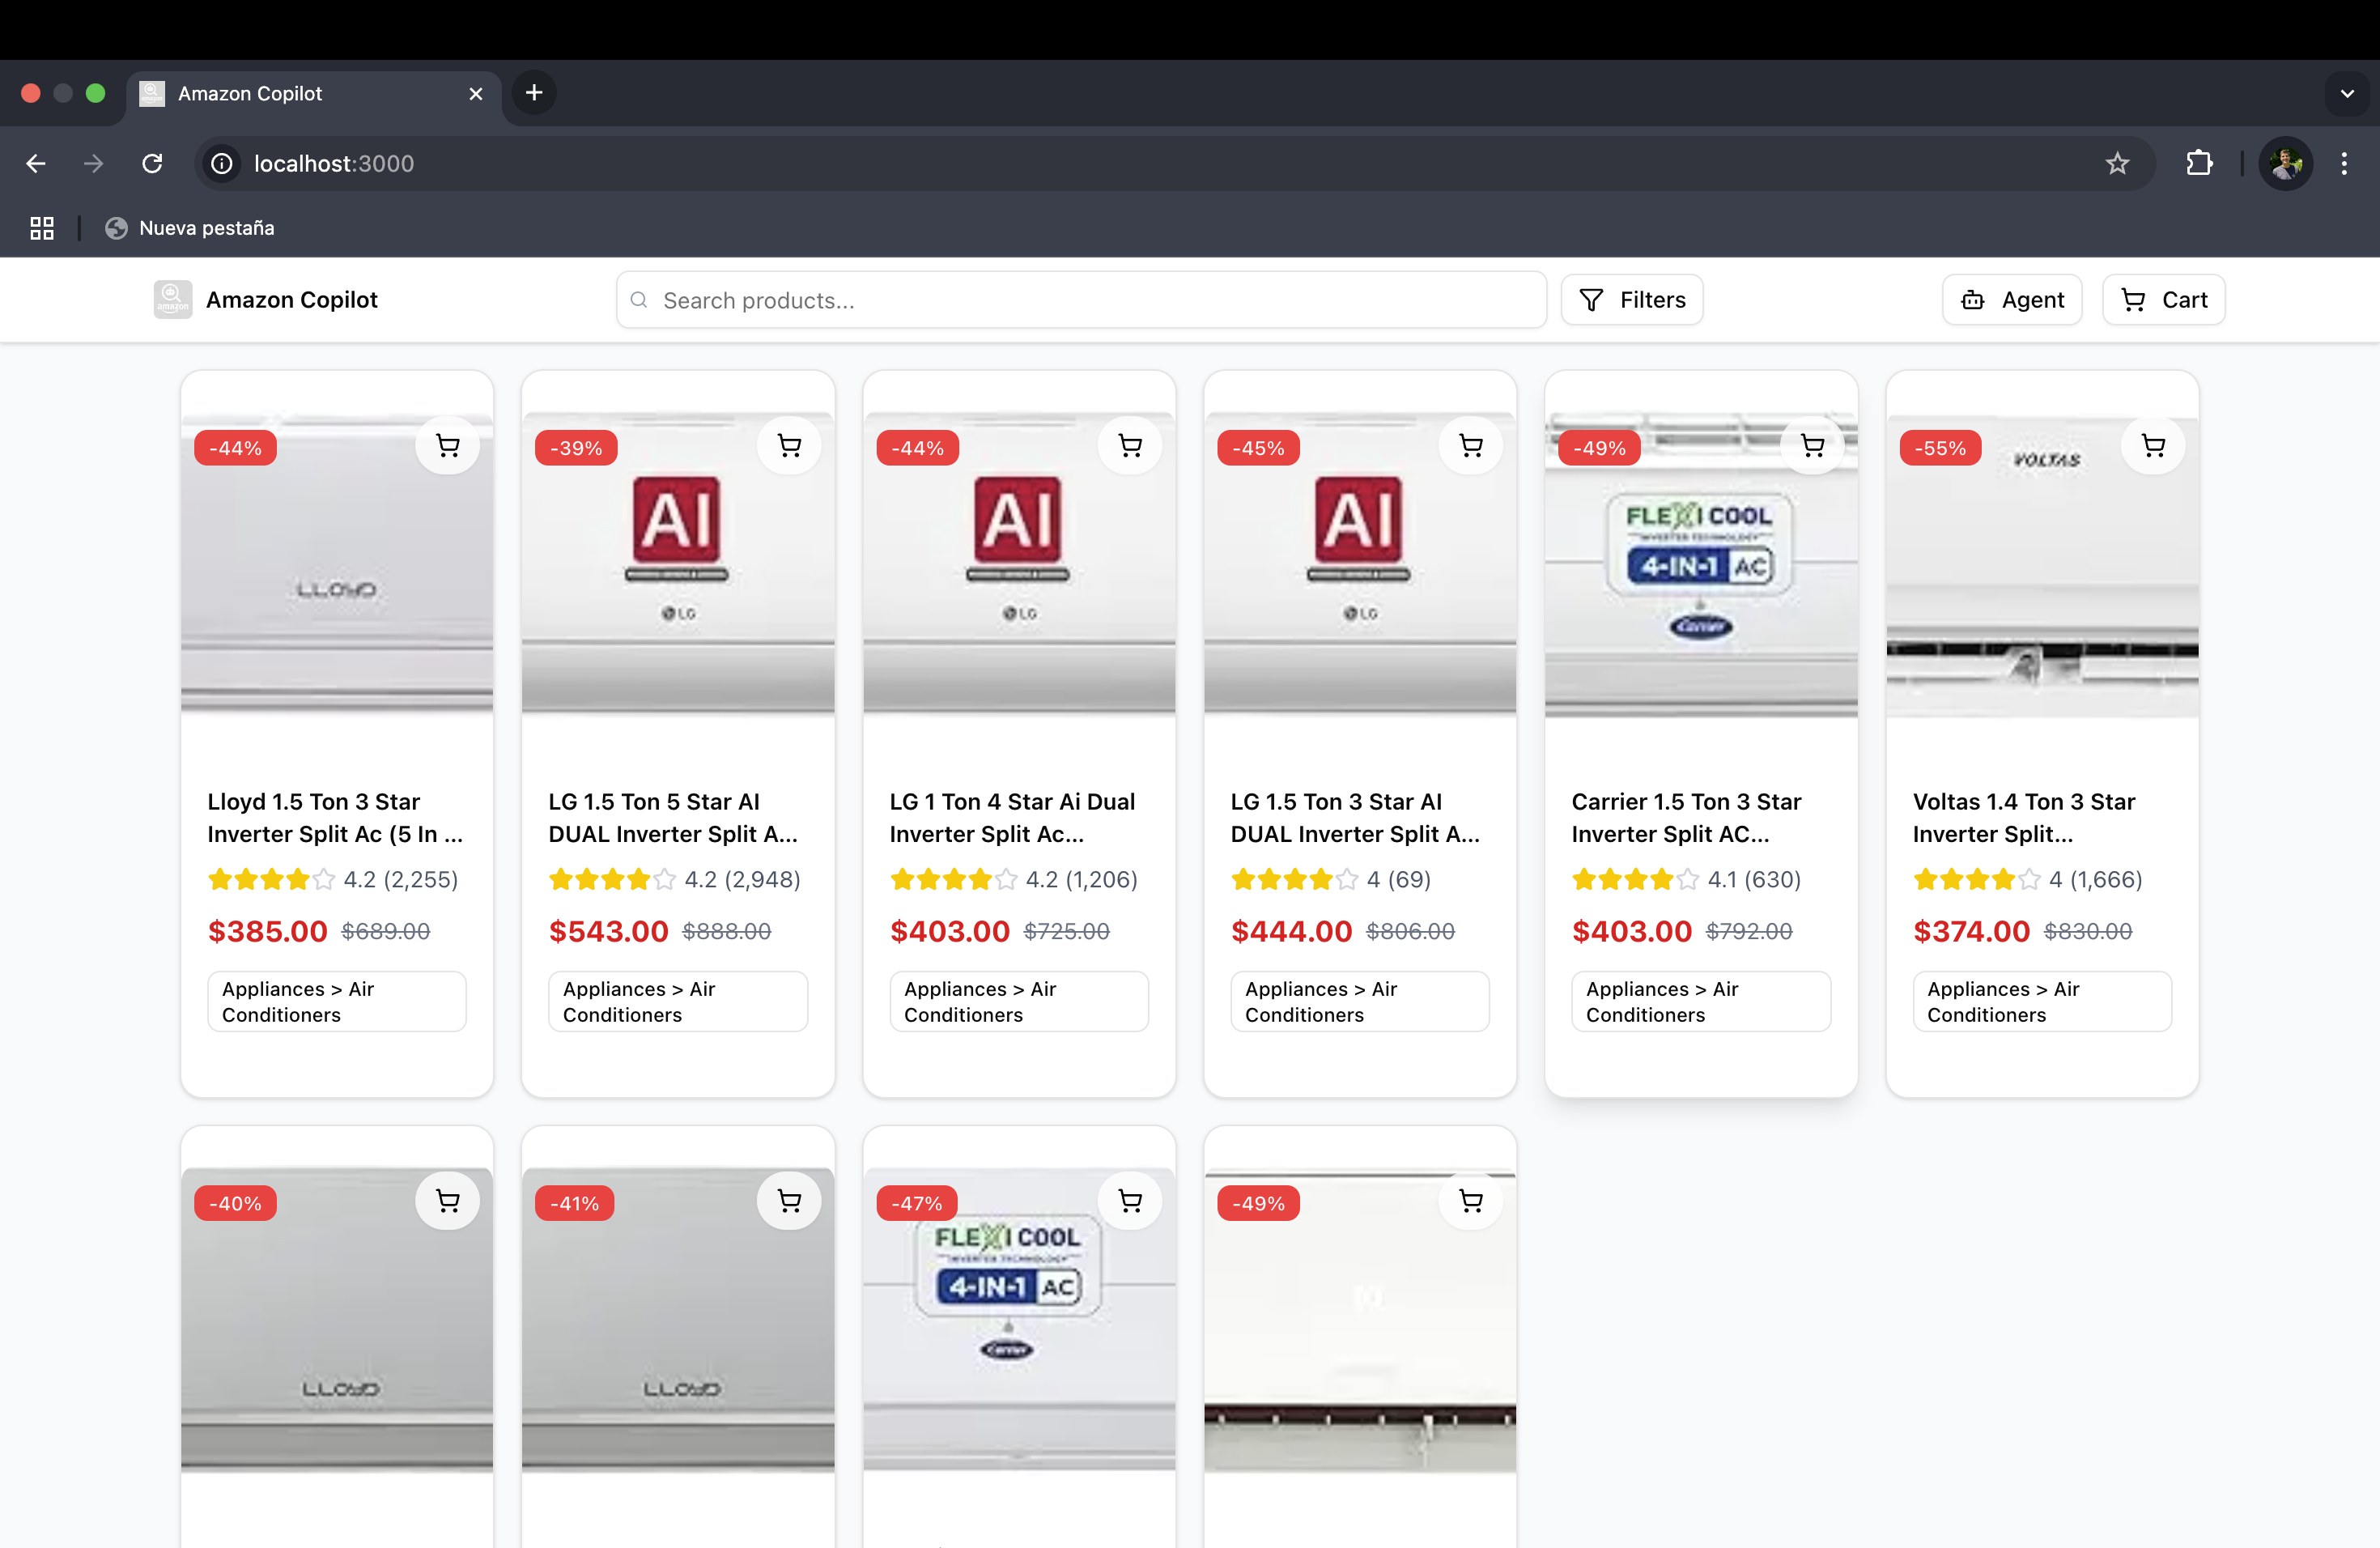
\includegraphics[width=0.8\textwidth]{home}
    \caption{Página principal - Catálogo de Productos}
\end{figure}

La interfaz incluye:
\begin{itemize}
    \item \textbf{Navbar superior}: Contiene el logo de la aplicación, barra de búsqueda y botones de navegación hacia el carrito y el asistente AI
    \item \textbf{Filtros dinámicos}: Panel lateral con categorías obtenidas dinámicamente del backend
    \item \textbf{Grid de productos}: Visualización en formato de tarjetas con información esencial (imagen, título, precio, descuento)
    \item \textbf{Paginación}: Controles para navegar entre páginas de resultados
\end{itemize}

\begin{figure}[H]
    \centering
    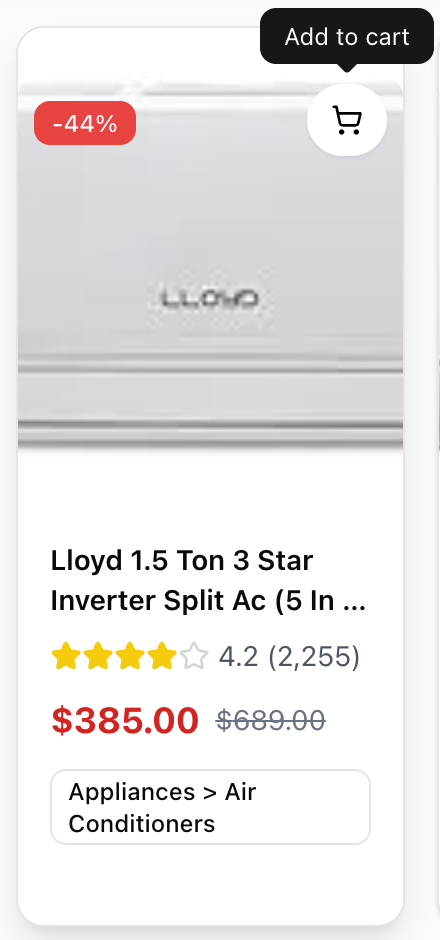
\includegraphics[width=0.45\textwidth]{product}
    \caption{Detalle de un producto en la página principal}
\end{figure}

\subsubsection{Página del Carrito}

La página del carrito (\textit{Cart}) proporciona una vista consolidada de los productos seleccionados y funcionalidades adicionales de recomendación.

\begin{figure}[H]
    \centering
    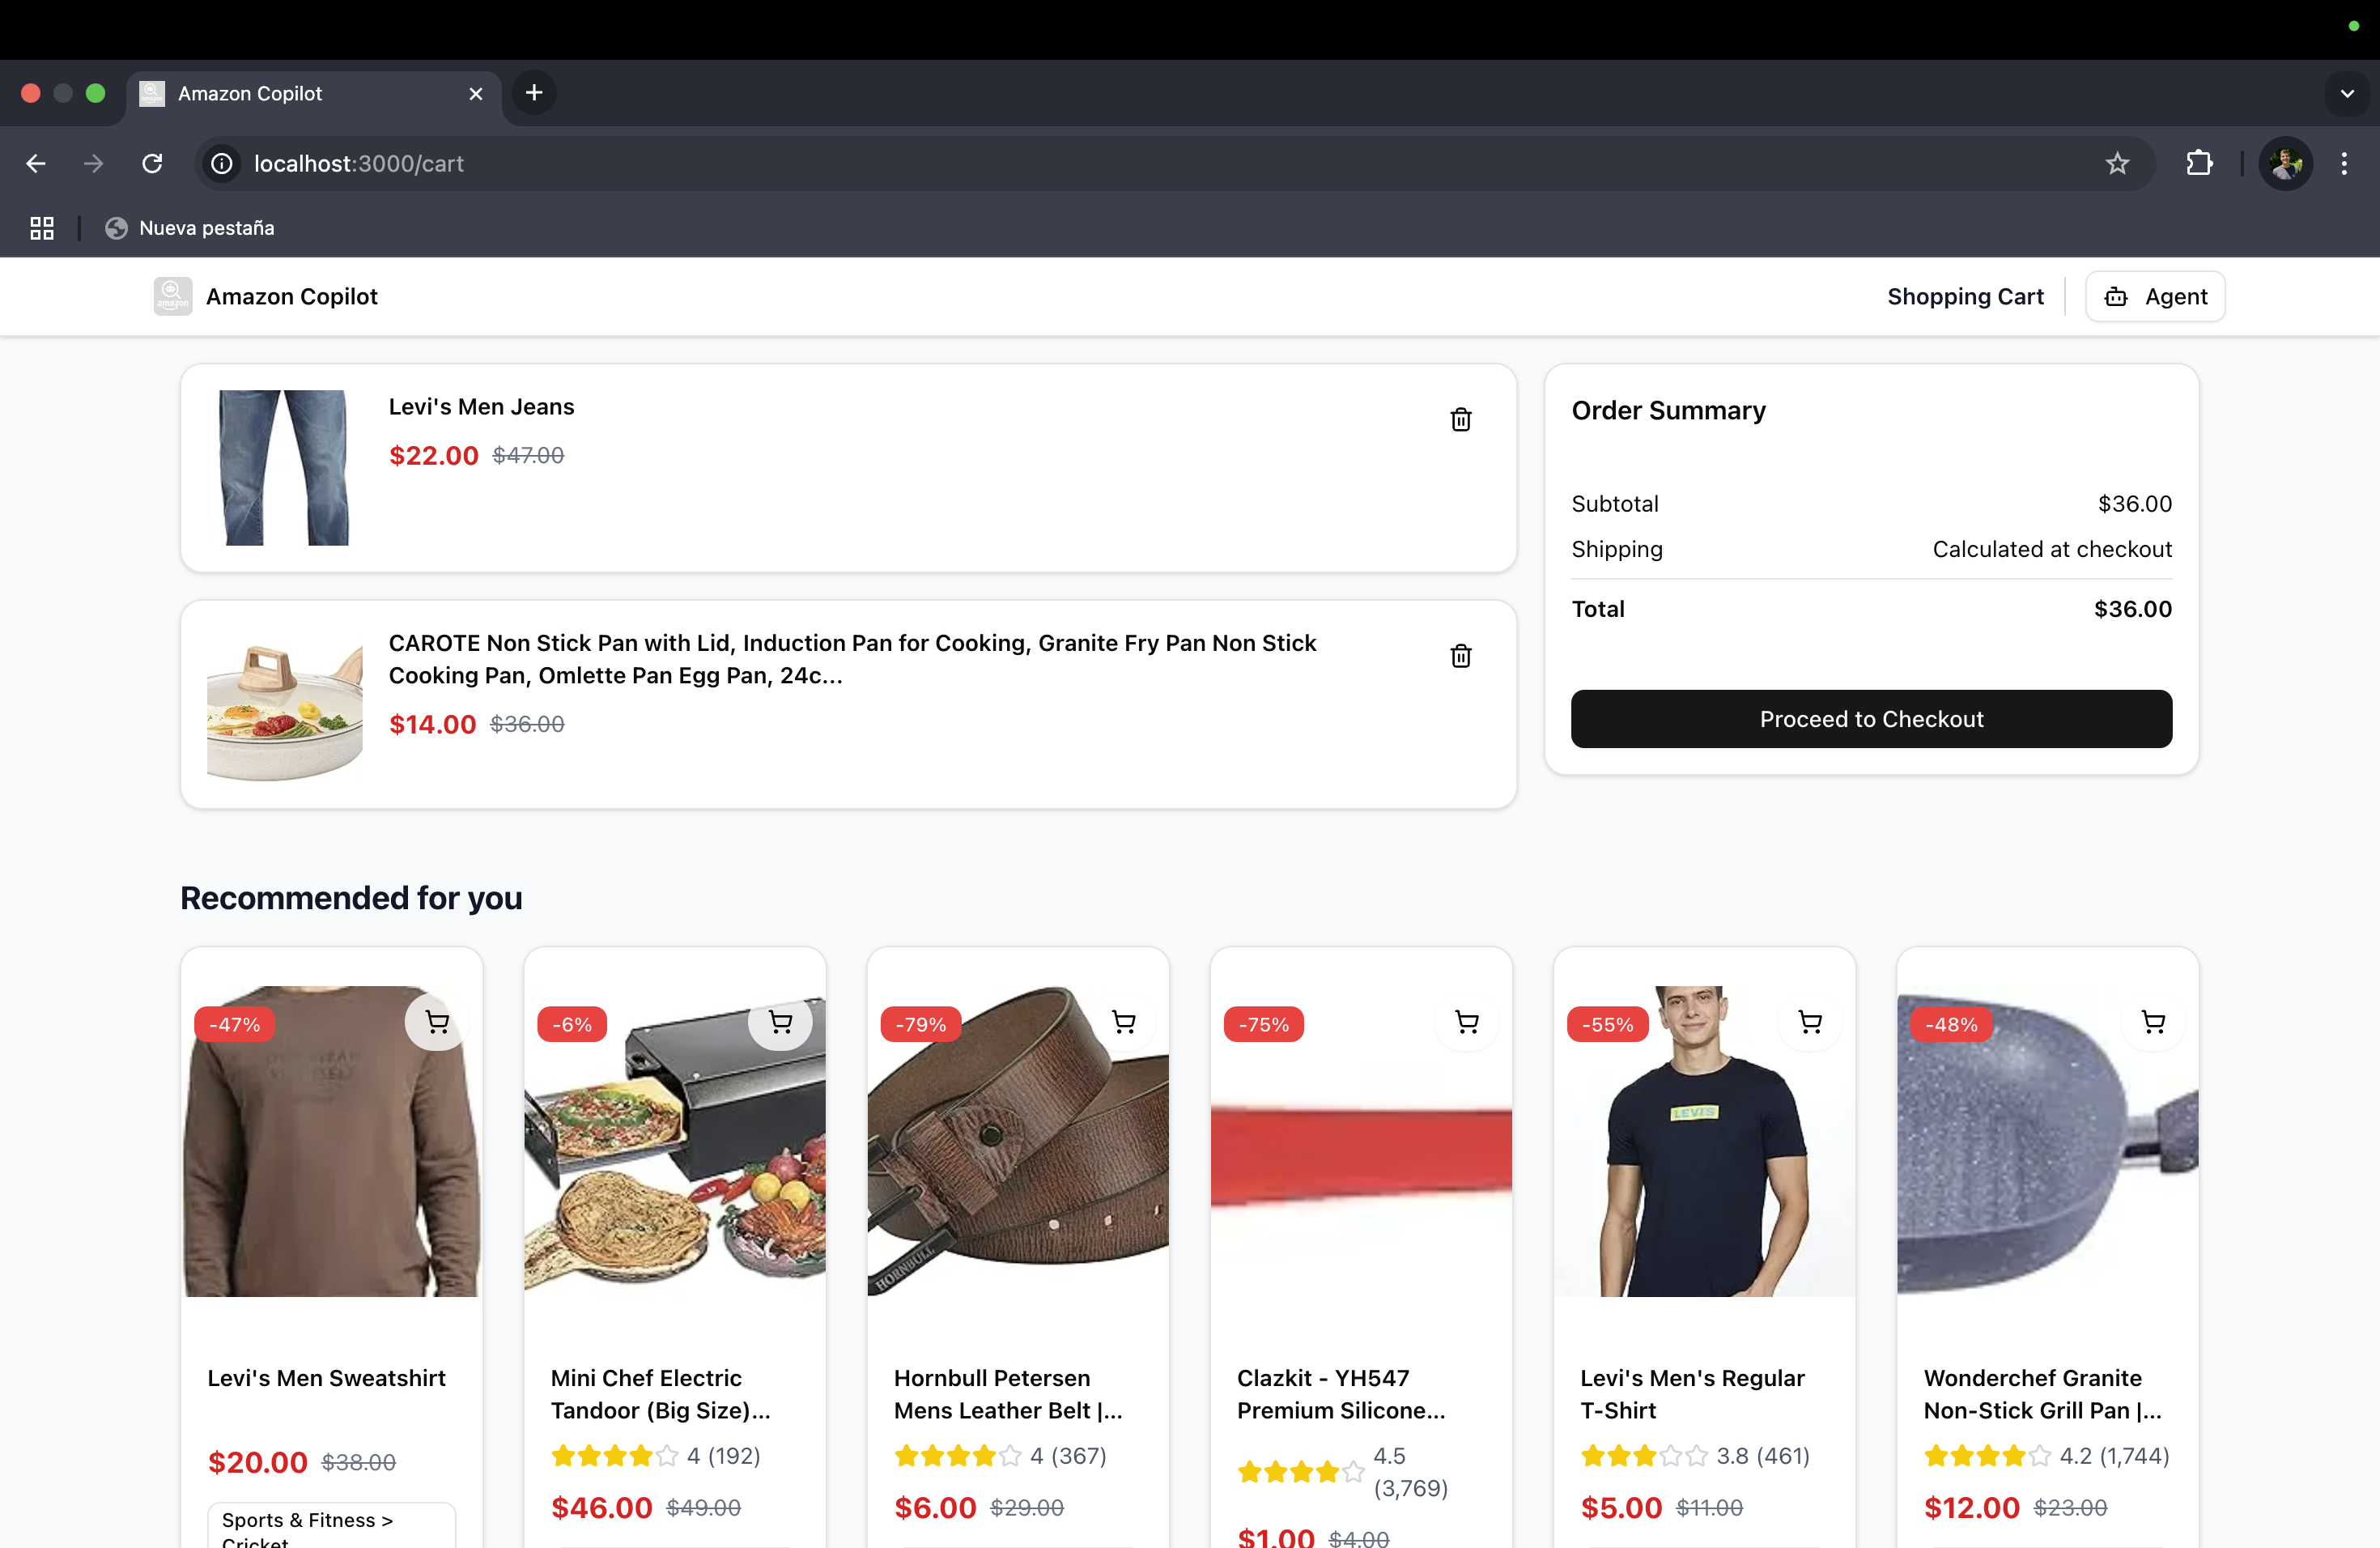
\includegraphics[width=0.8\textwidth]{cart}
    \caption{Página del carrito}
\end{figure}


Esta página se estructura en tres secciones principales:
\begin{itemize}
    \item \textbf{Lista de productos}: Muestra todos los items agregados al carrito con opciones de eliminación
    \item \textbf{Resumen de orden}: Panel lateral con el total de la compra y botón de checkout
    \item \textbf{Recomendaciones}: Sección inferior que sugiere productos relacionados basados en el contenido del carrito
\end{itemize}

\subsubsection{Página del Asistente AI}

La página del asistente (\textit{Agent}) implementa una interfaz de chat conversacional para asistir al usuario en sus consultas sobre productos.

\begin{figure}[H]
    \centering
    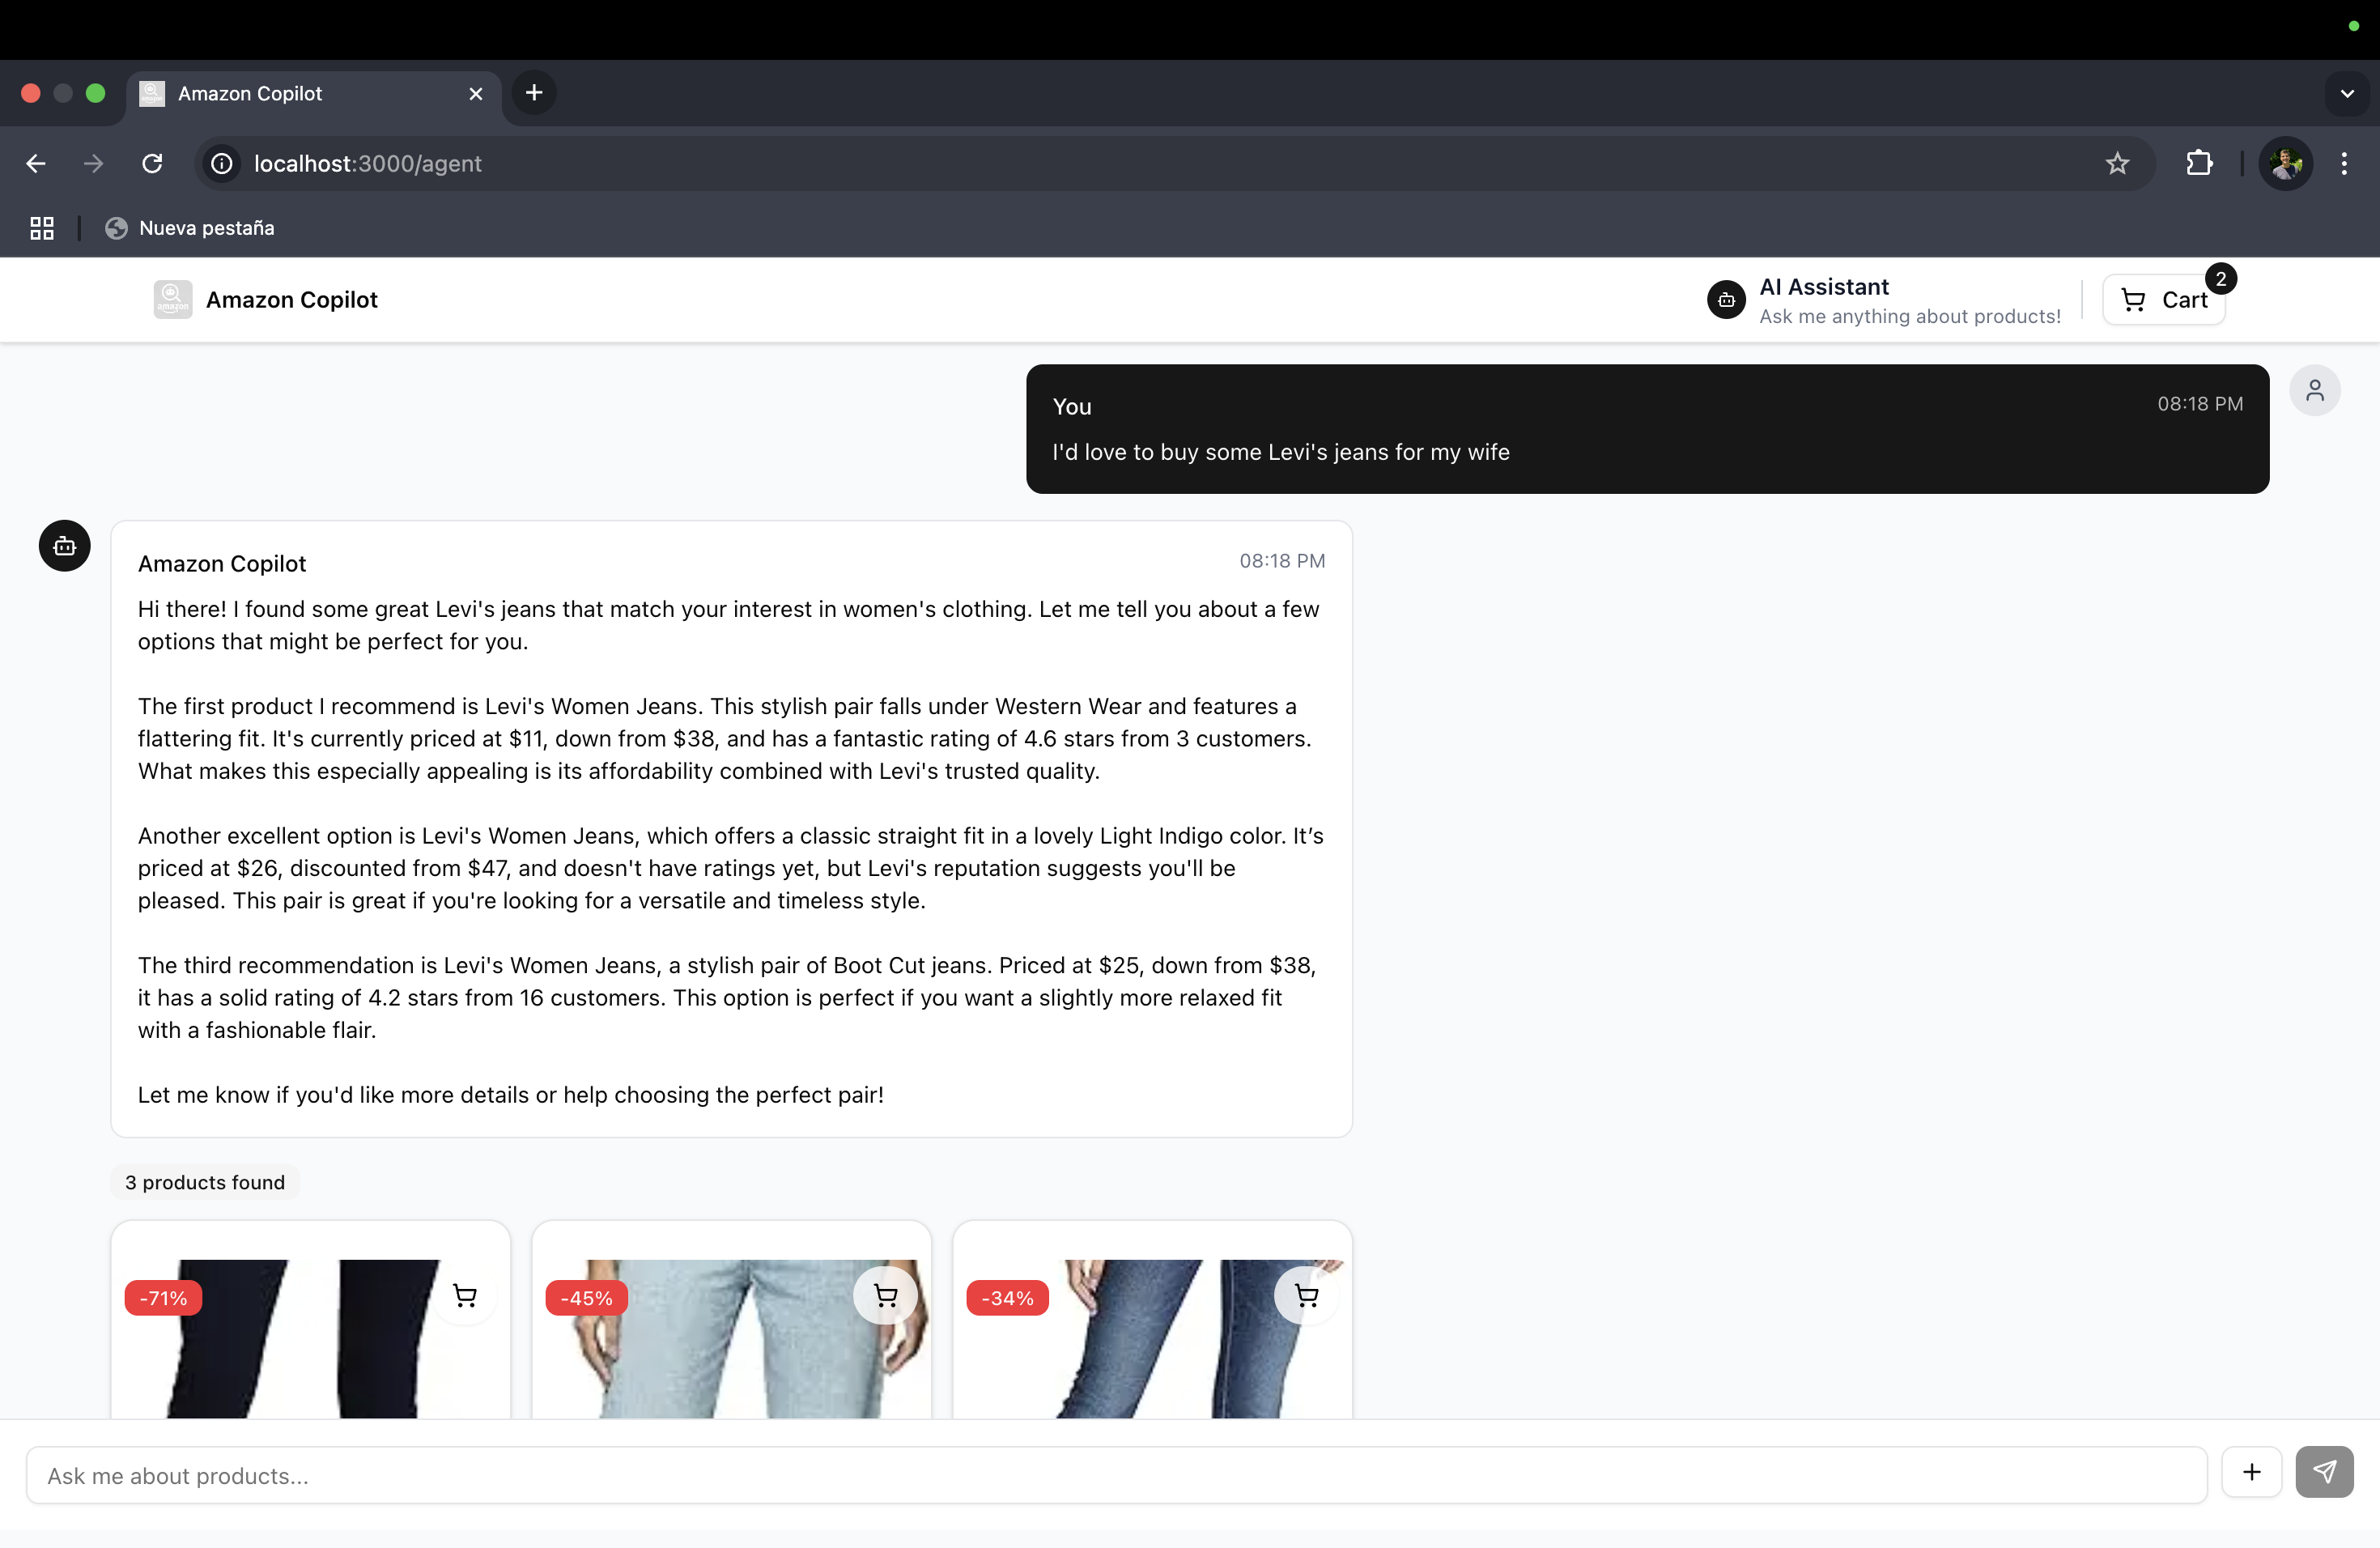
\includegraphics[width=0.8\textwidth]{agent}
    \caption{Página del asistente AI}
\end{figure}

Características principales:
\begin{itemize}
    \item \textbf{Interfaz de chat}: Diseño limpio con burbujas de mensaje diferenciadas por rol
    \item \textbf{Indicador de carga}: Feedback visual durante el procesamiento de mensajes
    \item \textbf{Productos sugeridos}: Visualización de productos recomendados por el asistente
    \item \textbf{Navegación contextual}: Enlaces directos a productos mencionados en la conversación
\end{itemize}

\subsection{Búsqueda y Filtrado Dinámico}

El sistema de búsqueda y filtrado implementa una arquitectura que optimiza tanto la experiencia del usuario como el rendimiento del backend.

\subsubsection{Filtros Dinámicos}

Los filtros de categorías se obtienen dinámicamente a través del endpoint de categorías, pero con una característica importante: las categorías disponibles se calculan en función de todos los productos existentes en la base de datos, no solo de los productos mostrados en la página actual.

\begin{figure}[H]
    \centering
    \begin{minipage}{0.45\textwidth}
        \centering
        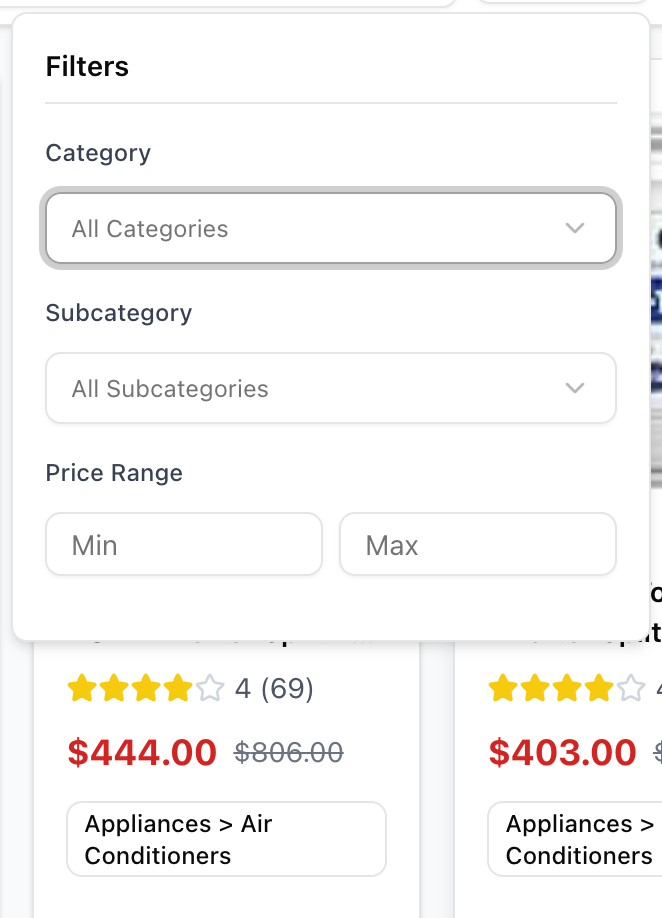
\includegraphics[width=\textwidth]{filters}
    \end{minipage}
    \hfill
    \begin{minipage}{0.45\textwidth}
        \centering
        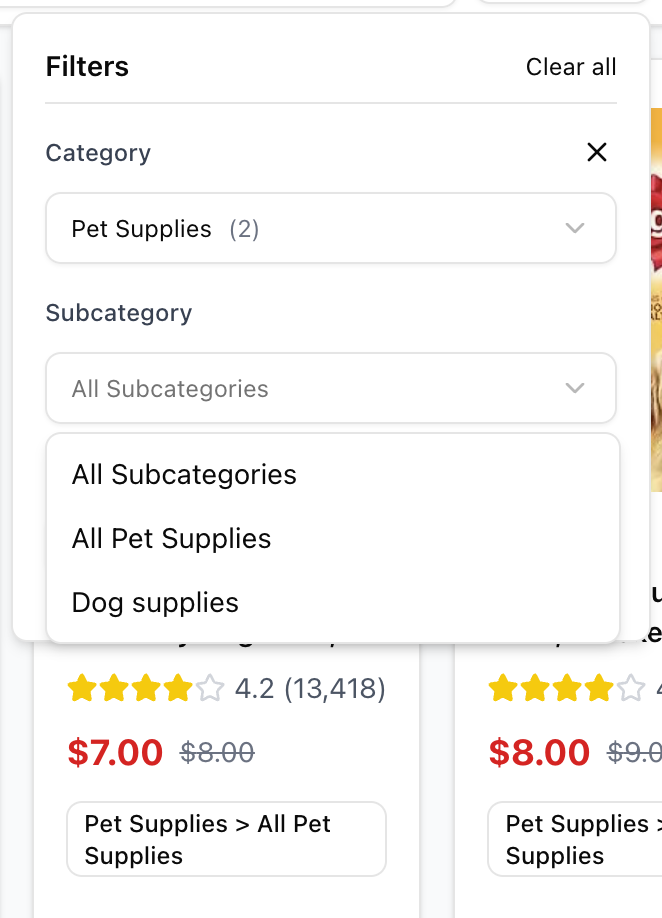
\includegraphics[width=\textwidth]{filters-2}
    \end{minipage}
    \caption{Panel de filtros}
\end{figure}

Esta implementación ofrece varias ventajas fundamentales:

\begin{itemize}
    \item \textbf{Filtrado en Backend}: Tanto los filtros como la paginación se procesan completamente en el servidor, garantizando que cada consulta se ejecute sobre la totalidad del catálogo de productos disponible
    \item \textbf{Consistencia}: Los filtros siempre reflejan la totalidad del catálogo disponible, independientemente de la página actual o los resultados mostrados
    \item \textbf{Precisión}: Evita situaciones donde un filtro no devuelve resultados debido a limitaciones de la página actual
    \item \textbf{Eficiencia}: El filtrado y paginación se realizan a nivel de base de datos, optimizando las consultas y reduciendo la transferencia de datos innecesaria
    \item \textbf{Escalabilidad}: La arquitectura permite manejar catálogos de gran tamaño sin impactar el rendimiento del frontend
\end{itemize}

El flujo de procesamiento garantiza que cada búsqueda, filtro o cambio de página resulte en una nueva consulta al backend que opera sobre el conjunto completo de productos, asegurando resultados precisos y consistentes en todo momento.

\subsubsection{Query Parameters y Reactividad}

La aplicación utiliza query parameters para triggerear nuevas consultas, implementando un sistema reactivo que actualiza automáticamente los resultados cuando el usuario modifica los filtros o la búsqueda.

\begin{figure}[H]
    \centering
    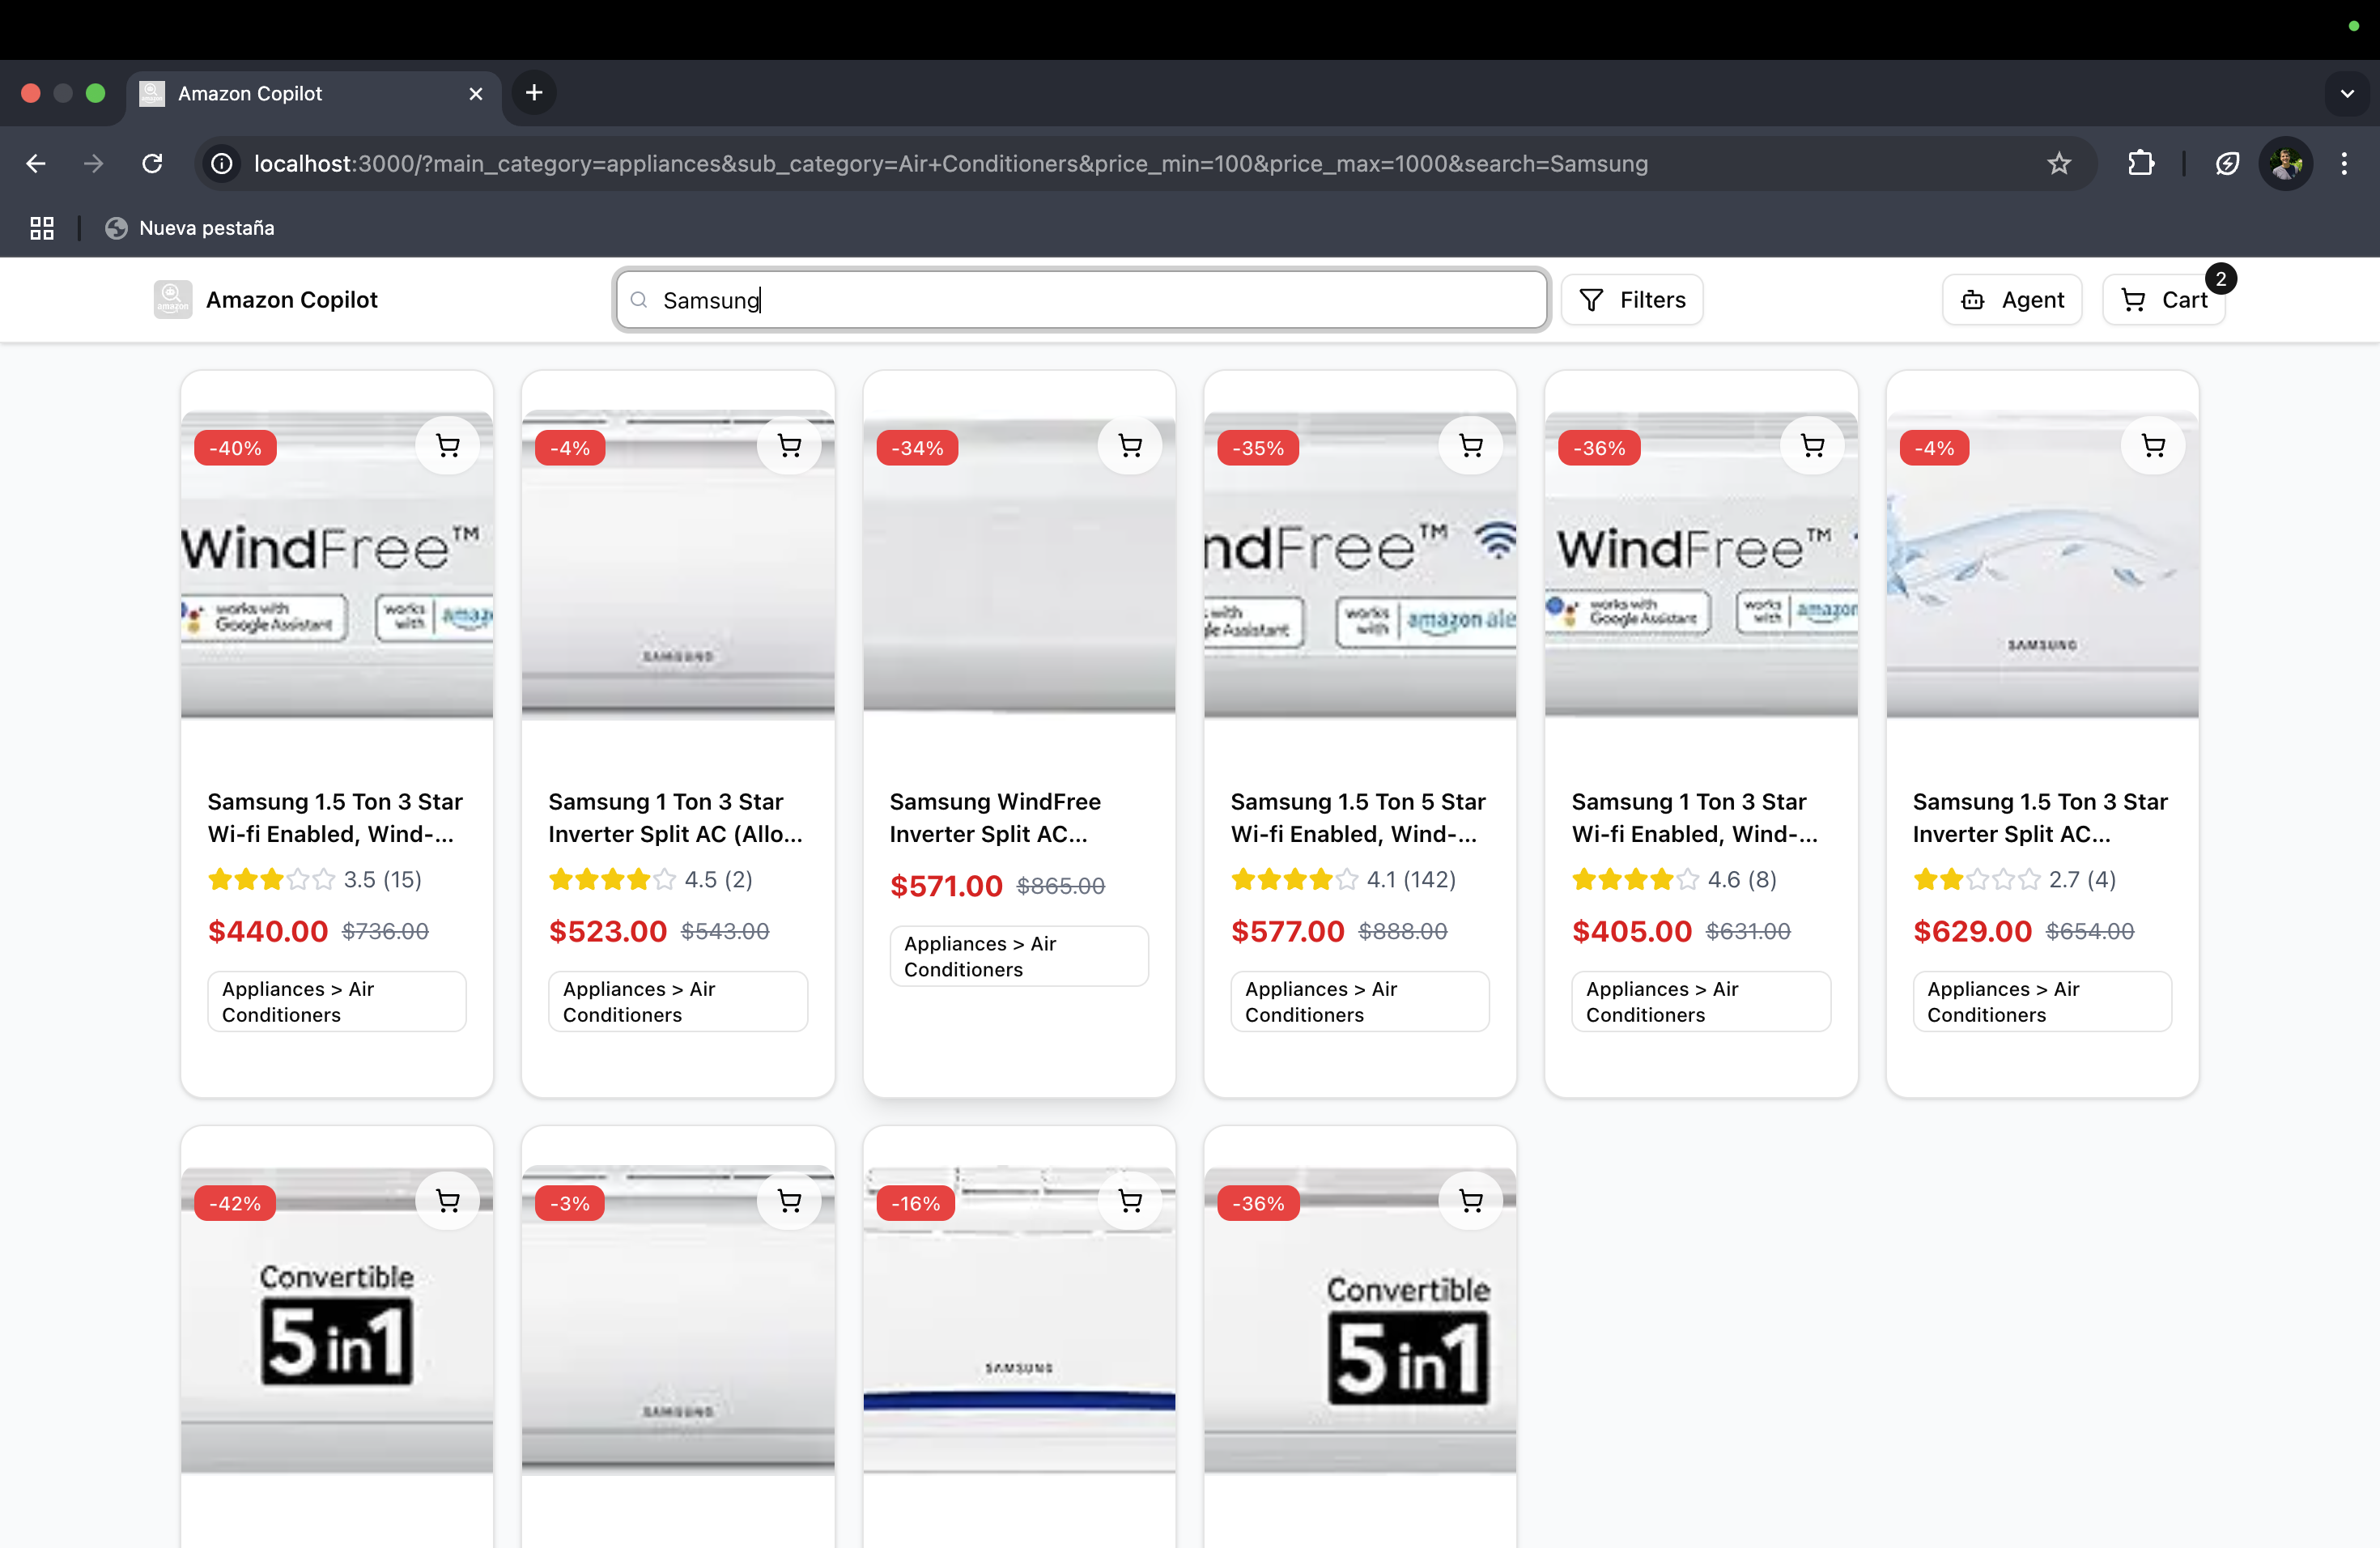
\includegraphics[width=0.8\textwidth]{query-parameters}
    \caption{URL con query parameters}
\end{figure}

El flujo de actualización funciona de la siguiente manera:
\begin{enumerate}
    \item El usuario modifica un filtro o realiza una búsqueda
    \item Los query parameters se actualizan en la URL
    \item Next.js detecta el cambio y re-renderiza la página
    \item Se ejecuta una nueva consulta al backend con los parámetros actualizados
    \item Los resultados se muestran al usuario
\end{enumerate}

Esta implementación ofrece ventajas adicionales:
\begin{itemize}
    \item \textbf{URLs compartibles}: Los usuarios pueden compartir resultados específicos simplemente copiando el enlace, ya que todos los parámetros de búsqueda y filtrado están codificados en la URL
    \item \textbf{Reproducibilidad}: Cualquier usuario puede reproducir exactamente los mismos resultados accediendo al enlace compartido
    \item \textbf{Bookmarking}: Los usuarios pueden guardar búsquedas específicas como favoritos en su navegador
\end{itemize}

\subsection{Arquitectura de Server Components y Suspense}

La aplicación aprovecha las capacidades avanzadas de Next.js 14, específicamente los Server Components y Suspense, para optimizar el rendimiento y la experiencia de usuario.

\subsubsection{Server Components}

Los Server Components permiten que la ejecución de queries comience desde el momento en que el navegador realiza la consulta al servidor web, no después de que se cargue el JavaScript en el cliente.

% [INSERTAR IMAGEN: Diagrama mostrando el flujo de Server Components vs Client Components]

Beneficios de esta arquitectura:
\begin{itemize}
    \item \textbf{Inicio temprano}: Las consultas se ejecutan en paralelo con la generación del HTML
    \item \textbf{Mejor SEO}: El contenido se renderiza en el servidor, mejorando la indexación
    \item \textbf{Menor JavaScript}: Reduce la cantidad de código que debe descargarse al cliente
    \item \textbf{Mejor rendimiento inicial}: La página se muestra más rápido al usuario
\end{itemize}

Además, la aplicación aprovecha los \textbf{Server Actions} de Next.js para operaciones que requieren interacción del servidor, como el envío de mensajes al asistente AI y la generación de recomendaciones de productos. Los Server Actions permiten ejecutar código del servidor directamente desde componentes del cliente, proporcionando una experiencia fluida sin necesidad de crear endpoints API separados.

\subsubsection{Suspense y Estados de Carga}

El componente Suspense se utiliza para proporcionar una experiencia de usuario fluida durante la carga de datos, implementando loading states que se muestran mientras se stremea el HTML con los datos.

\begin{figure}[H]
    \centering
    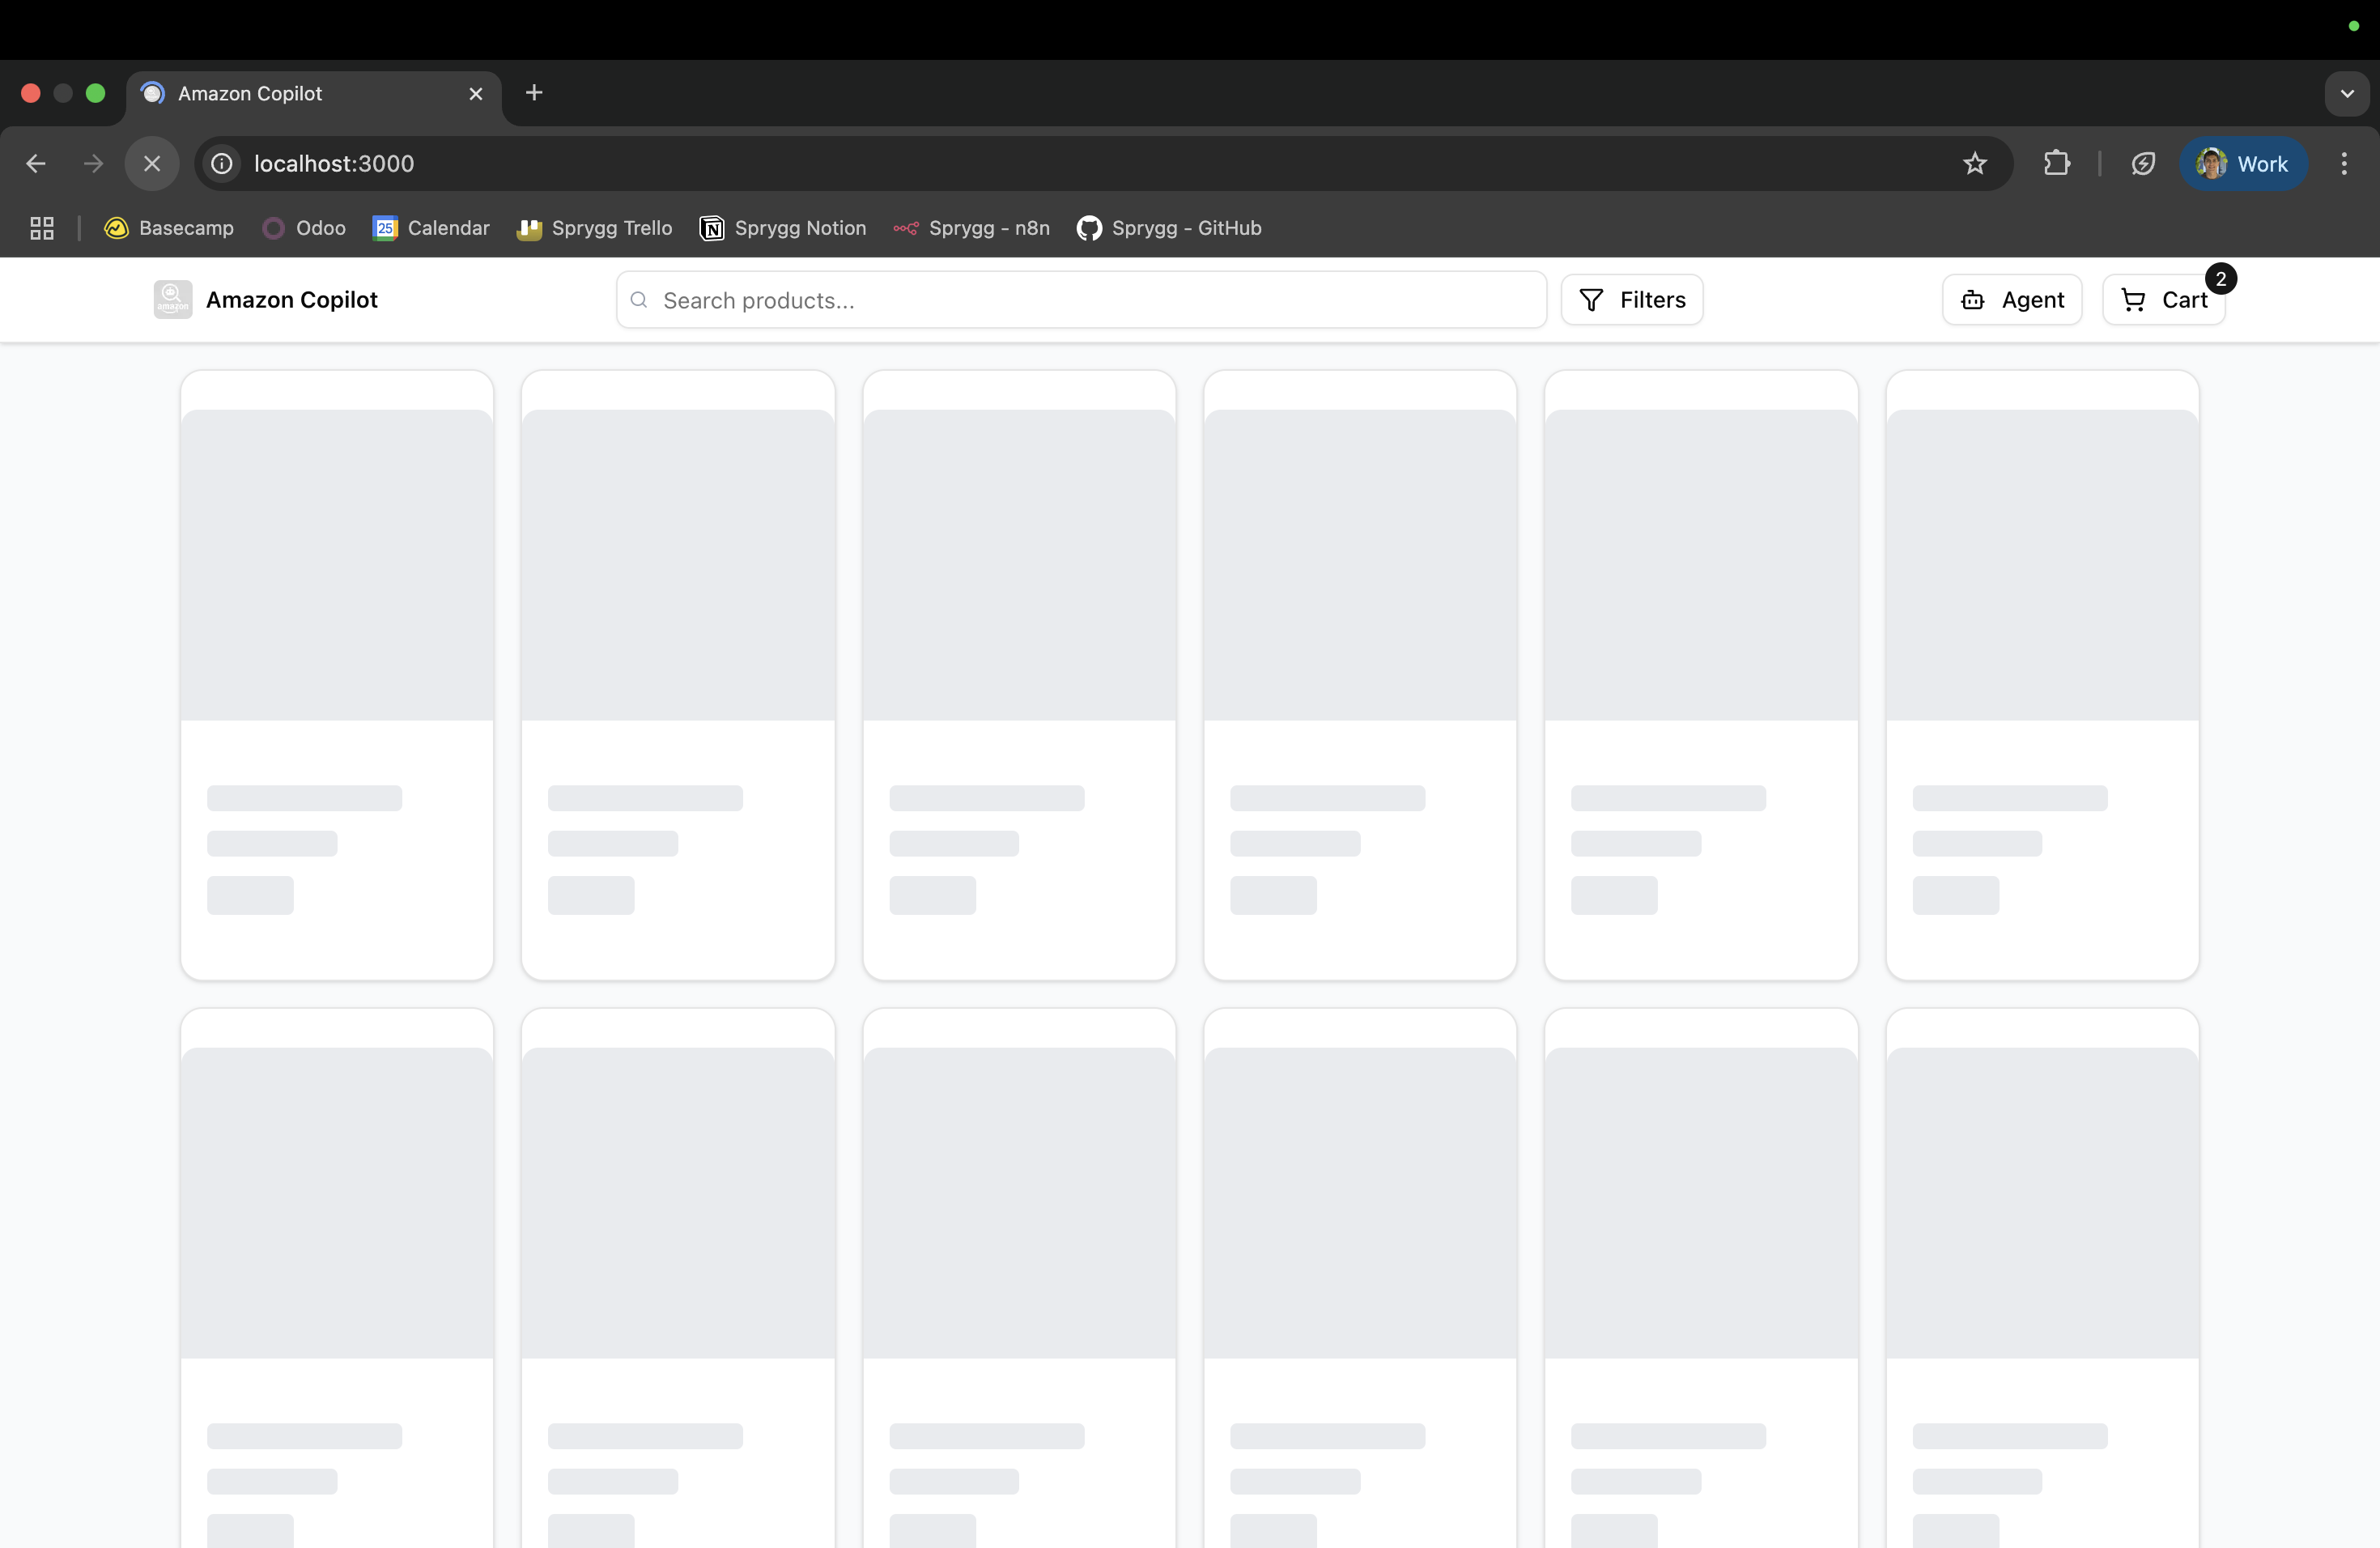
\includegraphics[width=0.8\textwidth]{skeleton}
    \caption{Estado de carga con Suspense}
\end{figure}


La implementación incluye:
\begin{itemize}
    \item \textbf{Skeleton loading}: Placeholders animados que simulan la estructura del contenido
    \item \textbf{Streaming progresivo}: Los datos se envían al cliente tan pronto como están disponibles
    \item \textbf{Transiciones suaves}: Los estados de carga se reemplazan sin interrupciones visuales
\end{itemize}

\subsection{Gestión de Estado con Contextos}

Para el carrito y el chatbot, se implementó un sistema de gestión de estado basado en contextos de React, combinado con almacenamiento local en el navegador.

\subsubsection{Contexto del Carrito}

El contexto del carrito maneja el estado de los productos seleccionados, almacenándolos en localStorage para persistencia entre sesiones.

Características principales:
\begin{itemize}
    \item \textbf{Persistencia local}: Los productos se mantienen entre recargas de página
    \item \textbf{Sincronización automática}: Cambios en el carrito se reflejan inmediatamente en toda la aplicación
    \item \textbf{Recomendaciones dinámicas}: Los productos del carrito se utilizan para generar recomendaciones personalizadas
\end{itemize}

\subsubsection{Contexto de Conversación}

El contexto de conversación gestiona el estado del chat con el asistente AI, implementando una estrategia híbrida de almacenamiento.

La implementación distingue entre dos tipos de datos:
\begin{itemize}
    \item \textbf{Mensajes}: Se almacenan en localStorage únicamente para su visualización en la interfaz
    \item \textbf{Identificador de conversación}: Se mantiene para preservar el contexto de la conversación en el backend
\end{itemize}

Esta separación permite:
\begin{itemize}
    \item \textbf{Contexto persistente}: El asistente mantiene memoria de mensajes anteriores
    \item \textbf{Experiencia fluida}: Los mensajes se muestran inmediatamente sin necesidad de recargar
    \item \textbf{Eficiencia de almacenamiento}: No se requiere una base de datos adicional para el estado
\end{itemize}

Esta arquitectura es especialmente adecuada para prototipos y aplicaciones de demostración, donde la simplicidad y velocidad de desarrollo son prioritarias sobre la persistencia a largo plazo de datos de estado.

\section{Expansión}

El presente capítulo traza una hoja de ruta para la evolución de Amazon Copilot, agrupando las iniciativas en tres grandes ejes: experiencia de usuario, calidad de las recomendaciones y robustez de la plataforma. Todas las ideas aquí expuestas son complementarias entre sí y pueden abordarse de forma incremental.

\subsection{Streaming de respuestas}

Implementar \textit{streaming} permitiría que el asistente enviase la respuesta de forma incremental—token a token—mediante \textit{Server-Sent Events} o \textit{WebSockets}.  
Esto traería dos ventajas principales:

\begin{itemize}
    \item \textbf{Percepción de inmediatez.} El usuario ve cómo el mensaje se «escribe» en pantalla, reduciendo la sensación de espera en consultas largas.
    \item \textbf{Interrupción inteligente.} Al recibir tokens en tiempo real, el cliente puede ofrecer al usuario la opción de cancelar, reformular o profundizar sin tener que esperar al final de la generación.
\end{itemize}

\subsection{Base de datos de telemetría y \textit{feedback}}

Registrar la interacción de los usuarios en una base de datos operacional abre la puerta a un ciclo virtuoso de mejora continua:

\begin{itemize}
    \item \textbf{Patrones de comportamiento.} Analizar clics, búsquedas y compras para detectar tendencias estacionales o hábitos de compra.
    \item \textbf{Re-entrenamiento de modelos.} Utilizar los datos recogidos para ajustar la ponderación entre embeddings densos y esparcidos, o para afinar los \emph{prompts}.
    \item \textbf{Personalización.} Mantener perfiles de preferencia (marcas, rangos de precio, colores) y aplicarlos en futuras consultas o recomendaciones.
    \item \textbf{Métricas de producto.} Medir \emph{CTR}, tasa de conversión y tiempo medio de respuesta para orientar decisiones de negocio.
\end{itemize}

\subsection{Embeddings de imágenes y búsqueda multimodal}

Extender el índice a vectores visuales dotaría al sistema de capacidades multimodales:

\begin{itemize}
    \item \textbf{Búsqueda inversa.} El usuario podría subir una foto o URL y recibir productos similares en forma, color o estilo.
    \item \textbf{Recomendaciones estéticas.} Combinar señal visual y textual para sugerir artículos que «combinen» con el carrito actual (p.\,ej. sets de ropa).
    \item \textbf{Comparación rápida.} Mostrar al usuario variaciones visuales (otros colores, modelos o diseños) sin depender solo de descripciones textuales.
\end{itemize}



\section{Conclusiones}

% TODO: Desarrollar conclusiones del proyecto


\newpage

\begin{thebibliography}{2}
    \raggedright

    \bibitem{Cursor}Cursor. (2024). \textit{Cursor: The AI-first code editor}. \url{https://www.cursor.com}

    \bibitem{Replit}Replit. (2024). \textit{Replit: The collaborative browser based IDE}. \url{https://replit.com}

    \bibitem{FastAPI}FastAPI. (2024). \textit{FastAPI: Framework web de alto rendimiento para APIs con Python}. \url{https://fastapi.tiangolo.com}

    \bibitem{Pydantic}Pydantic. (2024). \textit{Pydantic: Validación de datos para Python}. \url{https://docs.pydantic.dev/latest}

    \bibitem{LangGraph}LangGraph. (2024). \textit{LangGraph: Orchestration framework for building stateful, multi-actor applications with LLMs}. \url{https://www.langchain.com/langgraph}

    \bibitem{OpenAI}OpenAI. (2024). \textit{OpenAI: Creating safe AI that benefits humanity}. \url{https://openai.com}

    \bibitem{Qdrant}Qdrant. (2024). \textit{Qdrant: Vector Database}. \url{https://qdrant.tech/documentation/search-precision/reranking-hybrid-search}

    \bibitem{Amazon}Parab, L. (2023). \textit{Amazon Products Dataset}. Kaggle. \url{https://www.kaggle.com/datasets/lokeshparab/amazon-products-dataset/data?select=Amazon-Products.csv}

\end{thebibliography}

\end{document}
